\chapter{Background} \label{background}

\section{Introduction to mobile robotics}
%In this chapter, I am going to provide the scientific background of this thesis. 
The scientific and technological foundation of mobile robotics has evolved through research on various aspects of robot motion, environmental perception, mapping, and localization. This chapter provides an overview of the essential concepts underpinning autonomous navigation and scene reconstruction, which are crucial to the systems studied in this thesis. We explore mobile robotics, LiDAR SLAM and its visual counterparts VSLAM and visual-inertial odometry (VIO), and the emerging fields of photorealistic reconstruction, all of which contribute to the ability of robots to navigate and interact with their environment effectively.

%\section{Introduction to mobile robotics}

Mobile robotics focuses on the design, implementation, and control of autonomous robots that can navigate in dynamic, unknown environments~\cite{probabilistic_robotics}. The field intersects with various sub-disciplines in engineering, computer science, and AI, aimed at developing intelligent systems capable of movement without human intervention. The integration of sensors, actuators, and computational algorithms in mobile robots has led to significant advancements, particularly in mapping and localization. Early contributions in the field laid the groundwork for more sophisticated robotic platforms, emphasizing the need for reliable localization, obstacle avoidance, and path planning~\cite{introduction_to_autonomous_mobile_robots}.

\section{Odometry in mobile robots}

Odometry is a fundamental concept in mobile robotics that deals with the estimation of a robot's position and orientation over time as it moves through an environment. This process typically involves measuring changes in position based on the motion of the robot’s wheels. Odometry enables a robot to understand its incremental motion relative to a known starting point, providing essential information for navigation and positioning in environments where external localization sources (such as GPS) may be unavailable or unreliable. However, odometry alone cannot provide the location of the robot in a given map.

\subsection{Basics of odometry}

The traditional approach to odometry relies on wheel encoders, which measure wheel rotations to estimate the distance traveled. Using simple geometric relationships, the robot’s forward motion and changes in orientation can be calculated from these measurements. For differential drive robots, which have two wheels independently controlled on either side, changes in orientation are derived from the difference in distance traveled by each wheel. This is extended to omnidirectional platforms with multiple wheels or non-wheel-based odometry, depending on the robot's configuration~\cite{odometry_1996}.

Despite its simplicity and efficiency, wheel-based odometry is prone to cumulative error, particularly in environments where wheel slippage occurs due to uneven surfaces, loose materials, or sharp turns. These issues are more pronounced in outdoor or rugged terrains, where conventional odometry can yield highly inaccurate results without additional corrections~\cite{odometry_1996}.

\subsection{Error accumulation and correction in odometry}

Odometry errors in mobile robots are typically classified as systematic and non-systematic errors. Systematic errors arise from mechanical imperfections, such as unequal wheel diameters or axle misalignments, which introduce biases in the measurements. These can often be minimized by careful calibration and parameter tuning. Non-systematic errors, on the other hand, result from unpredictable factors like wheel slip, bumps, and surface irregularities. These errors are challenging to mitigate solely with encoder data, as they vary with the environment and the robot’s movements~\cite{odometry_1996}.

To correct these errors, sensor fusion techniques have been developed, integrating additional sensory data (e.g., inertial or visual data) to compensate for drift in wheel odometry. Sensor fusion algorithms, such as the Kalman Filter (KF)~\cite{kalman1960} and Extended Kalman Filter (EKF)~\cite{extended_kalman_filter}, have become standard tools in mobile robotics for filtering noise and improving the reliability of odometry-based position estimates. These probabilistic models enable the robot to maintain a statistically grounded estimate of its state by dynamically adjusting to sensor inputs and system uncertainties.

\subsection{Visual Odometry}

To overcome the limitations of traditional wheel odometry, researchers have developed Visual Odometry (VO), which uses cameras to estimate a robot’s position by tracking visual features across sequential frames. Visual odometry generally involves the following steps:

\begin{enumerate} 
    \item Feature Detection and Matching: Salient features, such as corners or edges, are detected in each camera frame, and corresponding features are matched in consecutive frames.
    \item Motion Estimation: From the matched features, the robot’s relative motion between frames is estimated using techniques like the Epipolar Geometry~\cite{epipolar_geometry} or Homography Transformation~\cite{homography_transformation} for planar surfaces.
    \item Optimization and Filtering: The motion estimates are then optimized and refined to minimize error and ensure continuity across frames~\cite{visual_odometry}.
\end{enumerate}

Two popular approaches to VO include monocular and stereo visual odometry:
\begin{itemize}
    \item Monocular Visual Odometry: This uses a single camera and estimates depth information through motion, based on the geometry between consecutive frames. Monocular VO is computationally efficient but lacks scale information, which can lead to scaling ambiguities~\cite{monocular_VO}.
    \item Stereo Visual Odometry: This employs two cameras, providing depth information directly from the disparity between the stereo images. Stereo VO is more accurate in terms of scale but requires higher computational resources and synchronization between cameras~\cite{stereo_VO}.
\end{itemize}

The robustness of VO depends on environmental factors such as lighting, texture, and dynamic objects. To address these challenges, modern VO systems often incorporate deep learning models to enhance feature extraction and improve motion estimates under challenging conditions~\cite{deepVO}.

\subsection{Visual-Inertial Odometry}

Visual-Inertial Odometry (VIO) is an extension of visual odometry that incorporates data from Inertial Measurement Units (IMUs)—sensors that measure accelerations and rotational velocities. By fusing visual and inertial data, VIO can provide a more robust estimate of the robot's trajectory, compensating for drift and error accumulation in environments with limited visual information or rapid motion.

Key components of VIO include:
\begin{enumerate}
    \item Preintegration of Inertial Data: IMU data is continuously integrated over time to estimate motion between frames, which is combined with visual data to provide a more stable trajectory.
    \item Non-linear Optimization: VIO systems often use non-linear optimization techniques to fuse the visual and inertial data, refining the robot’s pose estimates.
    \item Outlier Rejection: Given the inherent noise in IMU data and the potential for feature mismatches in visual odometry, outlier rejection techniques are essential to filter out erroneous data points~\cite{VIO}.
\end{enumerate}

Popular VIO frameworks, such as ROVIO (Robust Visual-Inertial Odometry)~\cite{robust_VIO}, VINS-Mono~\cite{vins_mono} and Spectacular AI's HybVIO~\cite{hybvio}, have demonstrated high accuracy and real-time performance in a wide range of robotic applications, from autonomous drones to ground vehicles. These systems rely on tight coupling of visual and inertial measurements, enabling robust odometry in diverse environments. A typical drawback in practice is the need for calibration of individual sensors which might be a tedious task. Luckily, there exist purpose-built cameras for such robotics tasks that are calibrated during production and their calibration parameters are stored in their firmware.

\subsection{Applications of odometry in mobile robotics}

Odometry is a foundational component in a variety of mobile robotic applications, enabling robots to navigate in complex environments, build maps, and interact with surroundings. Key applications include:
\begin{itemize}
    \item Autonomous Ground Vehicles: In autonomous ground vehicles, precise odometry is crucial for navigation and collision avoidance, particularly in indoor environments where GPS is unavailable. Odometry data aids in path planning and obstacle detection, ensuring safe and efficient navigation.
    \item Drone Navigation: Drones rely heavily on VIO due to their requirement for precise positioning during rapid maneuvers. VIO is effective in aerial applications, particularly indoors or in GPS-denied areas, enabling stable flight control and obstacle avoidance.
    \item Robotic Manipulation: In mobile manipulators, odometry is essential for coordinating the robot's position with its end effector movements, particularly in tasks requiring precision, such as assembly or inspection.
\end{itemize}

\section{Localization and mapping}

Localization and mapping are two essential, interconnected processes in mobile robotics that allow robots to navigate and understand their environment. Localization is the robot's ability to determine its position within a known map, while mapping is the process of creating a map of an unknown environment based on sensor data. These capabilities are crucial for autonomous navigation, enabling a robot to explore new spaces, recognize its location, and avoid obstacles.

Traditionally, localization and mapping were treated as separate problems, but the development of Simultaneous Localization and Mapping (SLAM)~\cite{slam} has integrated the two into a single framework, allowing a robot to localize itself while concurrently building a map of its surroundings. SLAM is now the dominant paradigm in mobile robotics, supporting diverse applications such as autonomous vehicles, drones, and industrial robots.

\subsection{Challanges in localization and mapping}

The localization and mapping processes involve several key challenges that must be addressed for effective operation in dynamic, real-world environments:
\begin{itemize}
    \item Data Association: Identifying and matching features in sensor data across different time steps is essential for accurate mapping. This is difficult in dynamic environments where objects may move or change appearance.
    \item Loop Closure: Detecting when a robot revisits a previously mapped location is critical for correcting drift in the map. Loop closure algorithms rely on feature recognition to identify previously seen areas, allowing the robot to refine its position and correct any accumulated error in its map~\cite{loop_closure}.
    \item Map Representation: The choice of map representation affects the accuracy and efficiency of both localization and mapping. Maps can be represented in various formats, including grid maps, feature-based maps, or topological maps, each with its advantages and limitations depending on the application~\cite{map_representations}.
    \item Computational Complexity: SLAM algorithms often require significant computational resources, especially in large-scale or complex environments. Balancing real-time performance with map accuracy and detail is a critical trade-off in SLAM development~\cite{slam_computational_complexity}.
\end{itemize}

\subsection{Simultaneous Localization and Mapping}

Simultaneous Localization and Mapping (SLAM) is the process by which a robot builds a map of an unknown environment while simultaneously localizing itself within that map. SLAM algorithms generally consist of three primary components: sensor data processing, state estimation and map optimization.

\begin{itemize}
    \item Sensor Data Processing: SLAM systems use data from sensors such as LiDARs, cameras and IMUs to obtain measurements of the robot’s surroundings. These sensors provide complementary data; for instance, LiDAR offers accurate distance measurements, while cameras capture visual features~\cite{slam_used_sensors}.
    \item State Estimation: SLAM algorithms estimate the robot's position and orientation by processing sensor measurements through probabilistic models like the Extended Kalman Filter (EKF)~\cite{extended_kalman_filter} or Particle Filters~\cite{particle_filter}. These models maintain and estimate the robot’s state over time, adjusting as new sensor data is acquired.
    \item Map Optimization: Map optimization refines the robot’s position and the map representation by minimizing error through techniques like pose graph optimization. Loop closure detection and correction are integral parts of this process, enabling the system to handle long-term drift and maintain an accurate map~\cite{map_optimisation}.
\end{itemize}

SLAM can be categorized by the type of sensors used and the mathematical models employed, as seen on Figure~\ref{fig:slam_categories}. It has popular variations including LiDAR-based SLAM, visual SLAM (VSLAM), and multi-sensor SLAM. Each of these approaches has unique advantages depending on the operating environment and computational constraints.

\FloatBarrier
\begin{figure}[htbp]
	\centering
	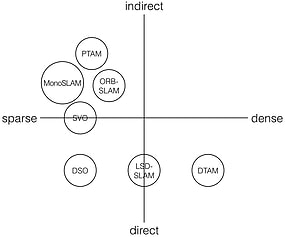
\includegraphics[width=100mm, keepaspectratio]{figures_jpg/slam_methods_categorization.jpg}
	\caption{Categories of SLAM methods}
	\label{fig:slam_categories}
\end{figure}
\FloatBarrier


\subsection{LiDAR-based SLAM}

LiDAR-based SLAM uses LiDAR sensors to measure distances by emitting laser beams and detecting their reflections~\cite{lidar}. This method creates precise maps of the environment, making it highly effective in indoor and outdoor settings with complex geometries. LiDAR-based SLAM algorithms, such as Hector SLAM~\cite{hector_slam} and Google’s Cartographer~\cite{google_cartographer}, leverage LiDAR's depth accuracy and robustness to ambient lighting changes, making them well-suited for autonomous ground vehicles, indoor robotics, and outdoor applications.

\subsection{Visual SLAM}

Visual SLAM (VSLAM) relies on cameras to capture visual features from the environment, using these features to localize the robot and create a map. VSLAM is particularly advantageous in environments where LiDAR may not be feasible or effective, such as environments containing dynamic objects, where a camera can be used to detect and exclude these objects. Key VSLAM techniques include:
\begin{itemize}
    \item Feature-based VSLAM: This approach detects and tracks visual features across consecutive frames. Algorithms like ORB-SLAM~\cite{orb_slam} and UcoSLAM~\cite{ucoslam} use these features to estimate motion and build a map.
    \item Direct VSLAM: Instead of relying on discrete feature points, direct VSLAM algorithms (e.g. DTAM~\cite{dtam} or LSD-SLAM~\cite{lsd_slam}) use the intensity of all pixels in an image to estimate motion and map the environment. This method is often more robust because it can identify edges on images, not just corners.
    \item Deep Learning-Augmented VSLAM: Recent advancements in deep learning have introduced VSLAM algorithms that leverage convolutional neural networks (CNNs) to improve feature extraction, depth estimation, and dynamic scene understanding. These enhancements are particularly valuable in challenging conditions where traditional feature-based methods struggle~\cite{deep_learning_vslam}.
    \item NeRF-based and Gaussian splatting-based SLAM: Recently, neural representations like Neural Radiance Fields (NeRFs) and Gaussian splatting have been adapted to SLAM, resulting in novel approaches such as NICE-SLAM~\cite{nice_slam}, NICER-SLAM~\cite{nicer_slam} or LoopSplat~\cite{loopsplat}. These methods leverage the strengths of implicit neural scene representations and probabilistic surface modeling to create detailed, dense maps with high photorealism.
\end{itemize}

\subsection{Multi-sensor SLAM}

Multi-sensor SLAM integrates data from various sensors (LiDARs, cameras, IMUs) to overcome the limitations of single-sensor SLAM systems. Multi-sensor fusion is particularly valuable in environments where no single sensor can provide reliable data alone. For example, IMUs can compensate for rapid movements that cause motion blur in cameras, while LiDAR provides accurate distance measurements in environments where visual data might be unreliable due to lighting conditions.

Multi-sensor SLAM algorithms typically use Kalman filters~\cite{kalman1960}, Particle filters~\cite{particle_filter}, or factor graphs~\cite{factor_graph} to fuse data and estimate the robot’s state with increased robustness. Approaches like QN-SAM-LIVO~\cite{qn_sam_livo} have successfully integrated LiDAR, visual and inertial data to achieve real-time, high-accuracy localization and mapping in diverse environments.

\subsection{Applications of localization and mapping in robotics}

The ability to localize and map autonomously has numerous applications in modern robotics, including:
\begin{itemize}
    \item Autonomous Vehicles: Self-driving cars require highly accurate maps of urban environments to navigate safely. LiDAR and camera-based SLAM systems provide the localization and situational awareness necessary for tasks like lane-following, obstacle detection, and traffic sign recognition~\cite{slam_for_autonomous_driving}.
    \item Drones and Aerial Robotics: For drones, localization and mapping are critical for stable flight control and collision avoidance. VSLAM and VIO techniques are widely used to enable drones to navigate in GPS-denied environments, such as indoors or densely forested areas~\cite{d2slam}.
    \item Service Robots: Indoor robots used in warehouses or hospitals rely on SLAM to navigate and interact with objects, providing services such as delivery, cleaning, and inspection. Grid-based or feature-based SLAM methods are commonly used in these applications~\cite{slam_for_service_robots}.
    \item Augmented Reality (AR) Applications: Visual-Inertial SLAM (VISLAM) is a key enabler for augmented reality (AR) technologies, including AR glasses and mobile platforms like ARCore~\cite{arcore} and ARKit~\cite{arkit}. These systems rely on VISLAM to accurately track device movement and maintain consistent spatial awareness in real-time. By fusing visual and inertial data, VISLAM enables AR applications to overlay virtual objects onto real-world scenes with high precision, supporting immersive experiences in gaming, navigation, and industrial design. Furthermore, its low-latency performance is crucial for delivering smooth, user-responsive interactions, making VISLAM indispensable in modern AR systems.
\end{itemize}


\section{Photorealistic reconstruction}

Photorealistic reconstruction refers to the process of creating highly detailed, lifelike 3D models of real-world environments, objects, or scenes. This is achieved by capturing fine visual details, textures, lighting, and spatial information that make the reconstruction indistinguishable from real life. The primary objective of photorealistic reconstruction is to generate virtual representations that maintain the visual fidelity and geometric accuracy required for applications like virtual reality (VR), augmented reality (AR), and, increasingly, mobile robotics. For robotics, these reconstructions are crucial for enhancing perception, improving decision-making in navigation, and enabling robots to interact effectively with their surroundings.

\subsection{Overview of 3D reconstruction}

3D reconstruction techniques in computer vision and graphics have evolved from simple geometric models to highly sophisticated, texture-rich models capable of photorealistic fidelity. The primary steps involved in 3D reconstruction include~\cite{3d_reconstruction_steps}:
\begin{enumerate}
    \item Data Acquisition: Data is captured using sensors like RGB cameras, depth sensors, LiDAR, or stereo cameras. Each sensor type contributes different information, such as color, depth, or surface structure, which together form the basis of a 3D model.
    \item Point Cloud Generation: A point cloud is generated from the sensor data, representing the 3D coordinates of points on object surfaces or environmental features. Point clouds provide the fundamental spatial structure of the scene.
    \item Surface Reconstruction: From the point cloud, surfaces are generated through techniques like triangulation, creating a mesh that connects these points into a continuous model. This process is refined to ensure smoothness, accuracy, and alignment with real-world geometry.
    \item Texturing and Shading: To achieve photorealism, textures and lighting effects are applied to the mesh. Texturing involves projecting captured images or textures onto the model surface, while shading uses lighting information to enhance realism, simulating shadow and reflection effects.
\end{enumerate}

Early 3D reconstruction methods relied heavily on explicit geometric modeling, but recent advancements in deep learning have introduced data-driven techniques that can capture finer details, handle occlusions, and generate more realistic scenes with less manual intervention. Neural networks have enabled significant breakthroughs in photorealistic reconstruction by directly learning 3D representations from visual data.

In robotics, photorealistic reconstruction is invaluable for creating detailed 3D maps of environments, especially in applications where accurate visual information is essential for effective robot-environment interactions. The following techniques are prominent in photorealistic reconstruction for robotics, each providing unique benefits depending on the required level of detail, processing power, and environmental complexity.

\subsection{Neural Radiance Fields}

Neural Radiance Fields (NeRFs) are a breakthrough in photorealistic reconstruction that use neural networks to generate high-fidelity representations of scenes from 2D images. NeRFs work by modeling the color and density of rays passing through a 3D space, which allows the model to synthesize novel views from arbitrary angles. The core of NeRF lies in its ability to represent complex scenes using a neural network, which estimates the appearance of each pixel by blending colors and densities along rays cast through a scene~\cite{nerf}.

NeRF uses a set of 2D images from multiple viewpoints as input. By training a neural network to predict the color and opacity along each viewing ray, NeRF learns a volumetric representation of the scene. This process enables it to reconstruct realistic lighting and textures that would be challenging to achieve with traditional 3D models.

NeRFs are highly beneficial in robotics for generating realistic and immersive 3D maps of an environment. This is particularly useful for simulated environments, where robots can be trained in photorealistic virtual spaces before being deployed in the real world. In scenarios like object manipulation or navigation in visually complex environments, NeRF-based reconstructions allow robots to make better-informed decisions by leveraging visual cues similar to those in real-world scenes.

Despite its photorealistic quality, NeRF is computationally intensive and requires significant GPU resources for training, making it challenging to implement in real-time applications. However, recent work has focused on optimizing NeRF for faster inference and deployment on mobile robotic platforms~\cite{nerfhub}. As seen on Figure~\ref{fig:nice_slam}, NiceSLAM~\cite{nice_slam} and PointSLAM~\cite{pointslam} uses NeRFs for map reconstruction.

\FloatBarrier
\begin{figure}[htbp]
	\centering
	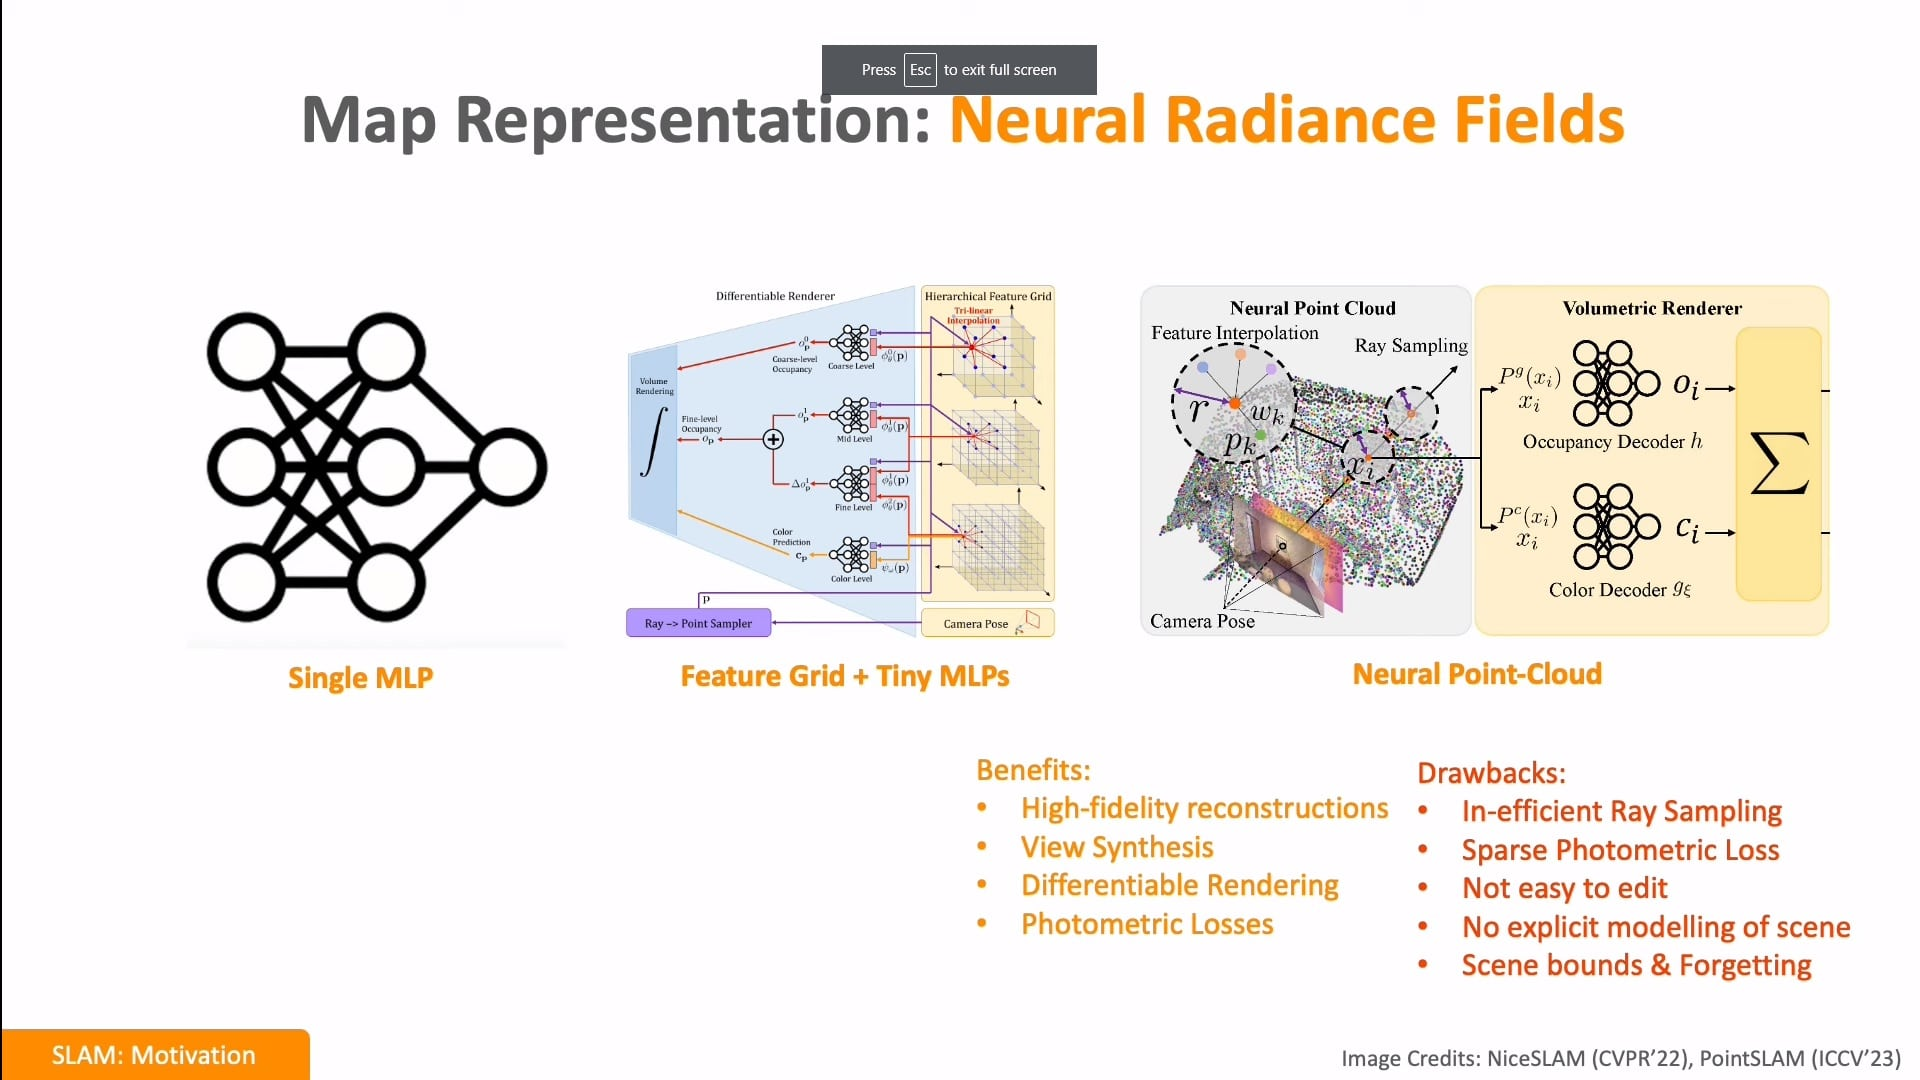
\includegraphics[width=150mm, keepaspectratio]{figures_jpg/nice_slam.jpg}
	\caption{Nice SLAM using NeRFs}
	\label{fig:nice_slam}
\end{figure}
\FloatBarrier


\subsection{Gaussian Splatting}

Gaussian Splatting is another novel approach to photorealistic reconstruction that models 3D scenes using Gaussian (3D ellipsoid) primitives with learnt view-dependent colors rather than point clouds or meshes. Each Gaussian represents a small, localized portion of the scene, allowing Gaussian Splatting to generate smooth and continuous reconstructions with high efficiency~\cite{3DGS}. Gaussian Splatting is much faster compared to neural networks, making it highly suitable for real-time applications in robotics.

In Gaussian Splatting, a 3D scene is approximated using Gaussian functions placed at points of interest in the environment. These Gaussians are blended to create a continuous surface, and their parameters are optimized to achieve high visual fidelity. By adjusting Gaussian parameters like mean, covariance, and intensity, Gaussian Splatting can represent scenes with high fidelity.

Gaussian Splatting is effective for large-scale mapping and outdoor applications, where computational efficiency and memory usage are critical. Drones, for example, can use Gaussian Splatting to rapidly construct and update 3D models of expansive outdoor environments. Gaussian Splatting’s efficient memory usage allows it to perform real-time updates, making it ideal for navigation, exploration, and environmental monitoring in mobile robots~\cite{active_splat} as seen on Figure~\ref{fig:gsplat_slam}. Recent researches are even targeting the problem of using even blurry datasets for reconstruction~\cite{gsplat_blur}.

\FloatBarrier
\begin{figure}[htbp]
	\centering
	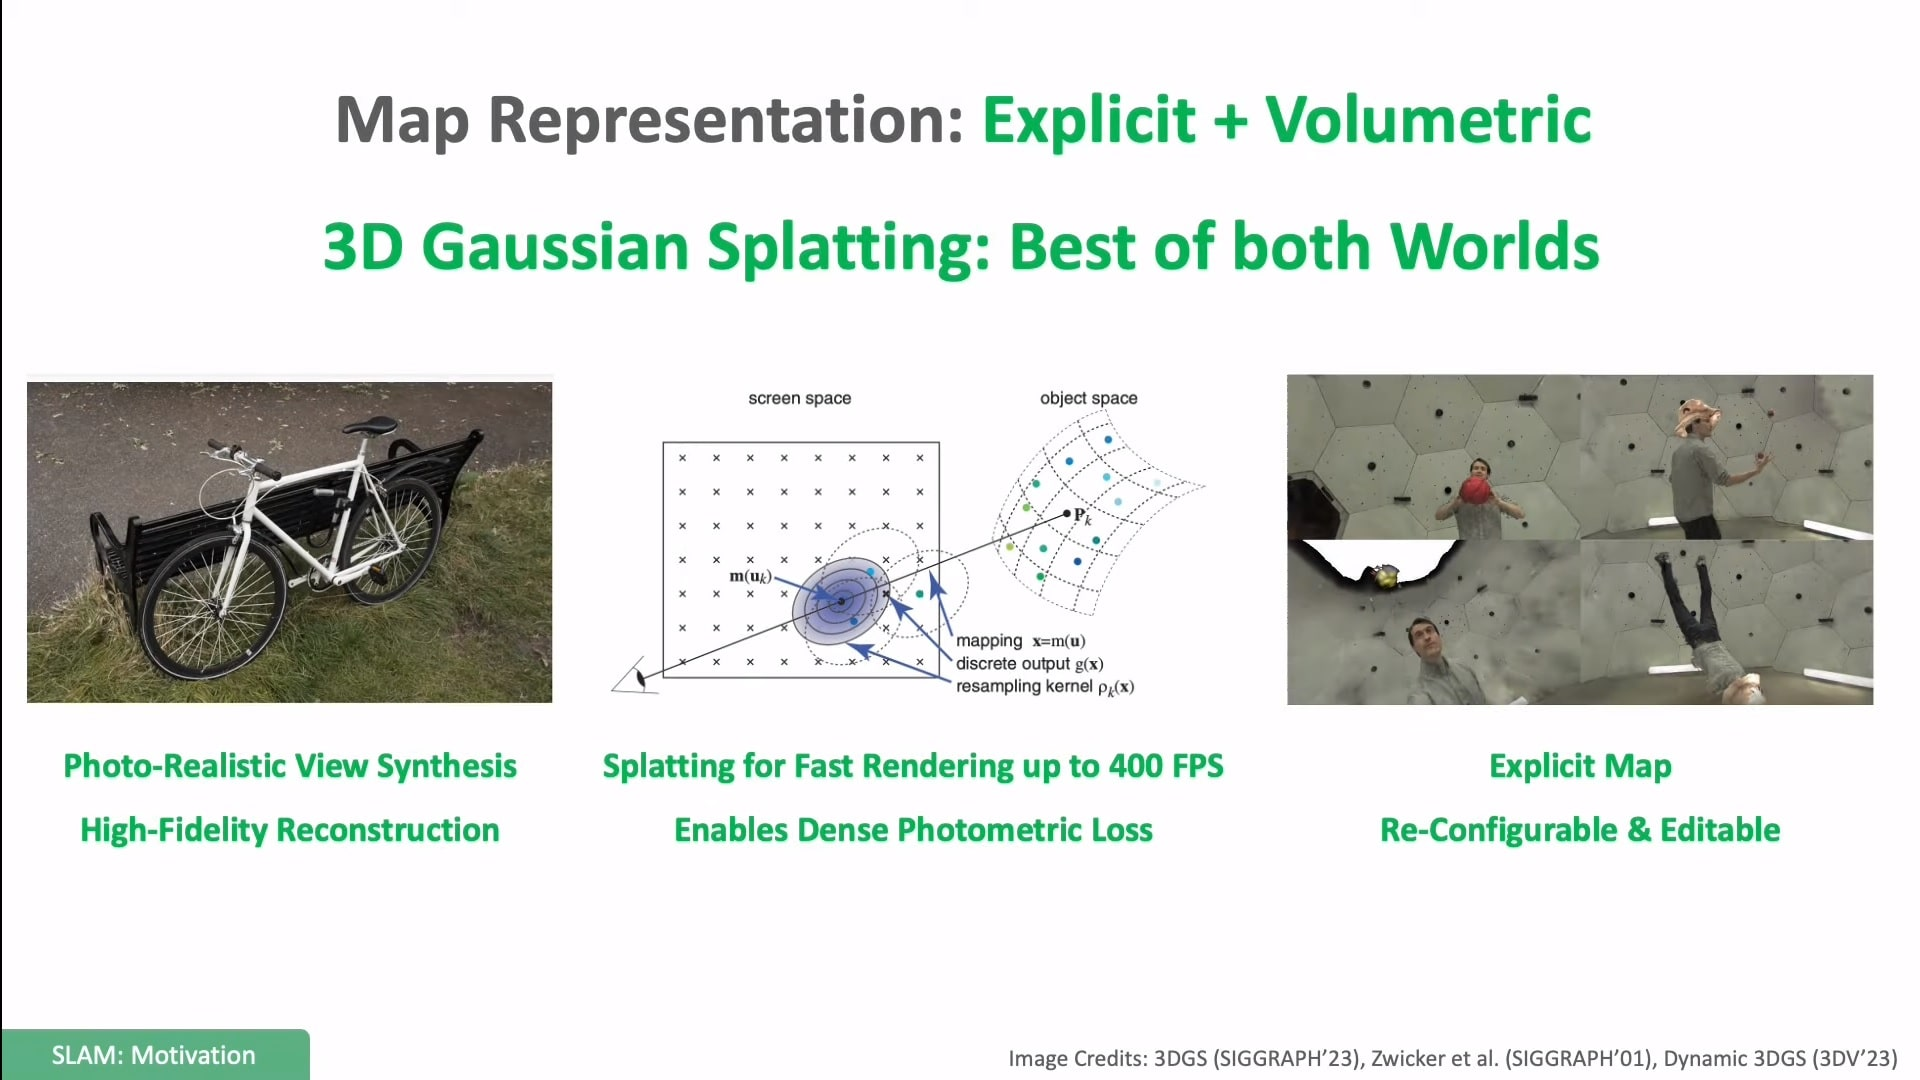
\includegraphics[width=150mm, keepaspectratio]{figures_jpg/gsplat_slam.jpg}
	\caption{Gaussian splatting in SLAM}
	\label{fig:gsplat_slam}
\end{figure}
\FloatBarrier


While Gaussian Splatting is efficient, it may not achieve the same level of photorealistic quality as NeRFs, especially in capturing fine texture details. However, for many robotic applications, its speed and memory efficiency make it a practical alternative. Recent studies show that it is possible to convert NeRFs' outputs to Gausssian Splattings' outputs and vice versa, making the computational requirements lower than training both from scratch~\cite{nerf_gsplat_convert}.

\subsection{Applications of photorealistic reconstruction in robotics}

Photorealistic reconstruction techniques are transforming the capabilities of mobile robotics by enhancing perception, enabling realistic simulation environments, and improving interactions with objects and scenes. Key applications of photorealistic reconstruction in robotics include:

\begin{itemize}
    \item Navigation and Path Planning: High-fidelity maps with realistic textures and lighting provide richer information for autonomous navigation. Robots can use photorealistic reconstructions to identify landmarks, avoid obstacles, and follow paths that are visually consistent with the real world~\cite{active_splat}.
    \item Simulation and Training: Simulations that incorporate photorealistic reconstructions allow robots to be trained in virtual environments that closely mirror real-world conditions. This is particularly useful in reinforcement learning, where robots can learn from interactions with highly realistic scenes, reducing the gap between simulated and real-world performance~\cite{reinforcement_learning_robot}.
    \item Object Recognition and Manipulation: Photorealistic 3D models of objects improve a robot's ability to recognize and interact with complex shapes. Robots can use NeRFs or Gaussian Splatting reconstructions to identify objects based on visual and spatial cues, facilitating tasks like grasping, sorting, and assembly~\cite{frodo}.
    \item Environmental Monitoring and Mapping: For applications like environmental monitoring, search and rescue, or archaeological documentation, photorealistic reconstructions capture important details, preserving visual information for analysis. Drones equipped with cameras can fly over large areas and create detailed maps, allowing scientists or first responders to assess environments in high fidelity~\cite{drone_3d_reconstruction}.
    \item Human-Robot Interaction: Robots used in collaborative settings, such as service robots or healthcare assistants, benefit from photorealistic models that help them understand and interpret human environments. For instance, a service robot in a home can navigate more effectively if it can distinguish furniture and objects with high accuracy. Recent studies show that it can even be used in healthcare where it is possible to create 3D reconstructions of slowly healing wounds~\cite{3d_reconstruction_wounds}.
\end{itemize}
